\documentclass[12pt, a4paper]{article}
\usepackage{fullpage}
\usepackage{amsmath}
\usepackage{graphicx}
\usepackage{natbib}
%\usepackage{epstopdf}
%\usepackage{chemstyle}
\title{Approaches and Examples for Modeling Microbially-Mediated Reactions}
\author{Guoping Tang}
\date\today{}

\begin{document}
\maketitle

\begin{abstract}
This document summarizes approaches and provides examples for modeling microbially-meditated reactions for the implementation of functions in PFLOTRAN for NGEE-Arctic fine/intermediate scale models. The kinetic rate is generally modeled by the Monod equation with various factors to account for thermodynamics, temperature, etc. In some applications (e.g., \cite{Wang2003283, Fang20096029, Yabusaki2007216, Riley2011}), the biomass is not tracked. When the biomass is tracked, the biomass synthesis reaction is either included (anabolic reaction, e.g., \cite{Luo2007129,Istok20101,rittmann2001environmental}) or not include (catabolic reaction, e.g., \cite{Jin20111,Li2009,bethke2007geochemical,Gu2010141}) in the redox reactions. The decay of the biomass is generally modeled with a first order decay, but without explicitly model the reactions. To complete the carbon cycle, the carbon incorporated into and decomposed from biomass may need to be explicitly included.
\end{abstract}

\section{Biomass Not Tracked}
When the biomass is not tracked (e.g., \cite{Wang2003283, Fang20096029, Yabusaki2007216, Riley2011}), the reaction rate is

\begin{equation}  
r = k_{max}\frac{m_D}{k_D + m_D}\frac{m_A}{k_A + m_A}\frac{k_I}{k_I + m_I}
\end{equation}

\begin{tabular}{ll}
$r$ & reaction rate for the redox reaction [$\mathrm{ML^{-3}T^{-1}}$] \\
$k_{max}$ & maximum rate coefficient [$\mathrm{ML^{-3}T^{-1}}$] \\
$m_{A}$ & electron acceptor concentration [$\mathrm{ML^{-3}}$] \\
$m_{D}$ & electron donor concentration [$\mathrm{ML^{-3}}$] \\
$m_{I}$ & inhibitor concentration [$\mathrm{ML^{-3}}$] \\
$k_{A}$ & electron acceptor half saturation concentration [$\mathrm{ML^{-3}}$] \\
$k_{D}$ & electron donor half saturation concentration [$\mathrm{ML^{-3}}$] \\
$k_{I}$ & inhibitor half saturation concentration [$\mathrm{ML^{-3}}$] \\
\end{tabular}
\\
\emph{Example 1. Sulfate reduction with acetate as the electron donor}
\\
The sulfate reduction reaction is
\begin{center}
$\mathrm{CH_3COO^- + SO_4^{2-} = 2 HCO_3^- + HS^-}$
\end{center}

The parameters are: $k_{max} = 1 \times 10^{-10}$ M/s, $k_A = 3.9 \times 10^{-5}$ M, $k_D = 5 \times 10^{-6}$ M, initial acetate = 1 mM, sulfate = 1.5 mM. The simulation results are shown in Figure \ref{Fig1} using PHREEQC.

\begin{figure}[h]
\centering
\includegraphics[width=0.5\textwidth]{ex1.eps}%
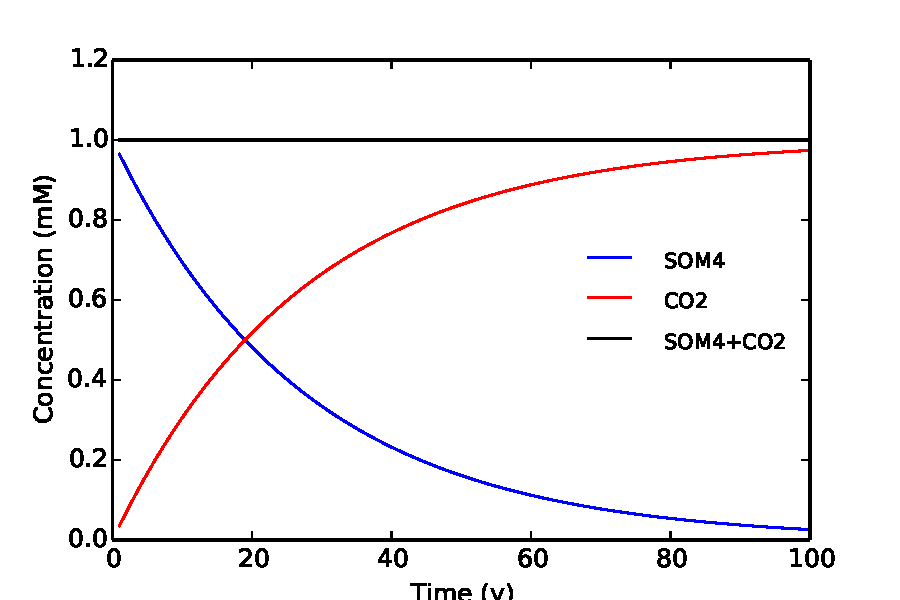
\includegraphics[width=0.5\textwidth]{ex2.eps}
\caption{PHREEQC results for Example 1 (left) and 2 (right)}
\label{Fig1}
\end{figure}

\emph{Example 2. Sulfate reduction with acetate as the electron donor and with nitrate inhibition}
\\
The nitrate reduction reaction is
\begin{center}
$\mathrm{CH_3COO^- + 1.6 NO_3^{-} + 0.6 H^+ = 2 HCO_3^- + 0.8 N_2 + 0.8 H_2O}$
\end{center}

The parameters for nitrate reduction are: $k_{max} = 3 \times 10^{-9}$ M/s, $k_A = 2.3 \times 10^{-6}$ M, $k_D = 1 \times 10^{-6}$ M, $k_I = 1 \times 10^{-6}$ M, the initial nitrate concentration = 0.5 mM. The parameters for sulfate reduction are identical to Example 1. The simulation results are shown in Figure \ref{Fig1}

\section{Catabolic Reaction with Monod Growth}
This approach includes a redox reaction, a cell synthesis reaction, and a decay reaction. However, the cell synthesis, and decay reactions are often not explicitly accounted for (\cite{Jin20111,Li2009,bethke2007geochemical,Gu2010141}). As the growth and decay of biomass are part of the carbon and nitrogen cycle, we need to consider explicitly including these reactions. However, the representation of biomass, growth and decay reactions are not widely used. A treatment was included in \cite{Wang2012} for a microbial-enzyme-mediated carbon decomposition model. 

The reaction rate for the redox reaction, for example,
\begin{center}
$\mathrm{CH_3COO^- + SO_4^{2-} = 2 HCO_3^- + HS^-}$
\end{center}
is
\begin{equation}  
r = \mu_{max}x\frac{m_D}{k_D + m_D}\frac{m_A}{k_A + m_A}\frac{k_I}{k_I + m_I}F_TF_{\theta}F_{pH}
\end{equation}

with
\\
\begin{tabular}{ll}
$\mu_{max}$ & maximum rate coefficient [$ML^{-3}T^{-1}$] \\
$x$ & biomass [$ML^{-3}$] \\
$F_{T}$ & thermodynamic factor \\
\end{tabular}

\begin{equation}  
F_T = 1 - exp\left(-\frac{\Delta G_A - \Delta G_C}{\chi RT}\right)
\end{equation}

\begin{tabular}{ll}
$\Delta G_A$ & energy available from the redox reaction \\
$\Delta G_C$ & energy saved by the functional group \\
$\chi$ & average stoichiometric number \\
$R$ & gas constant \\
$T$ & absolute temperature \\
\end{tabular}

\begin{equation}  
\Delta G_A = - \Delta G_T^0 - RT ln\prod{a_i^{\nu_i}}
\end{equation}

\begin{equation}  
\Delta G_C = m_{ATP} \Delta G_P
\end{equation}

\begin{tabular}{ll}
$\Delta G_T^0$ & standard Gibbs free energy change \\
$a_i$ & activity of reactants \\
$\nu_i$ & stoichiometric coefficient \\
$m_{ATP}$ & ATP yield \\
$\Delta G_P$ & the phosphorylation energy \\
\end{tabular}

The growth rate is

\begin{equation}  
dx/dt = -Yr
\end{equation}

\begin{tabular}{ll}
$Y$ & yield coefficient \\
\end{tabular}

The first order decay rate is

\begin{equation}  
dx/dt = Dx
\end{equation}

\begin{tabular}{ll}
$D$ & first order decay rate coefficient \\
\end{tabular}

\emph{Example 3. Sulfate reduction with acetate as the electron donor} \\
This example is extended from \cite{bethke2007geochemical}. 
A solution, initially sterile, contains 500 mM NaCl, 20 mM $\mathrm{CaSO_4}$, 2 mM $\mathrm{FeCO_3}$, and 1 mM $\mathrm{NaCH_3COO}$. Its pH is buffered to 7.2. At t = 0, the solution is inoculated with enough of the sulfate reducers to bring the initial biomass, expressed in terms of the dry weight of the cells, to 0.1 mg/L. The solution is incubated for three weeks.

The reaction is 

\begin{center}
$\mathrm{CH_3COO^- + SO_4^{2-} = 2 HCO_3^- + HS^-}$
\end{center}

$\chi$ = 5, $\Delta G_P$ = 45 kJ/mol, m = 1, therefore, 
\begin{equation}  
F_T = 1 -\left(\frac{Q}{K}\right)^{1/5} exp\left(\frac{9}{RT}\right)
\end{equation}
 
Sulfide produced from sulfate reduction is expected to precipitate with ferrous iron to form mackinawite (FeS), a precursor to pyrite ($\mathrm{FeS}$), with reaction.

\begin{center}
$\mathrm{FeS + H^+ = Fe^{2+} + HS^{-}}$
\end{center}

with log K = -3.6 at 25 $^\circ$C. The yield coefficient Y is 4.3 g/mol.

We consider four simulation cases:

Case 1: no acetate for biomass synthesis, no biomass decay

Case 2: first order decay at rate coefficient $\mathrm{D = 10^{-7}}$ 1/s 

Case 3: biomass synthesis from acetate

For each mole of sulfate reduction $\mathrm{CH_3COO^- + SO_4^{2-} = 2 HCO_3^- + HS^-}$, Y mole biomass is synthesized following $\mathrm{2.5 CH_3COO^- + 2.5 H^+ \rightarrow C_5H_7O_2N}$. $\mathrm{C_5H_7O_2N}$ is used to represent the biomass.

Case 4: biomass synthesis from acetate, and decay to produce $\mathrm{CO_2}$ following  $\mathrm{C_5H_7O_2N \rightarrow 5 CO_2}$

The simulation results are shown in Figure \ref{Fig2}.

\begin{figure}[h]
\centering
\includegraphics[width=1.0\textwidth]{ex3c.eps}
\caption{PHREEQC results for Example 3}
\label{Fig2}
\end{figure}

\section{Anabolic Reaction with Monod Growth}
An anabolic reaction often combines an electron donor (reduction) half reaction, e.g., 
\begin{center}
$\mathrm{ \frac{1}{8}CO_2 + \frac{1}{8}HCO_3^- + H^+ + e^- = \frac{1}{8}CH_3COO^- + \frac{3}{8} H_2O}$,
\end{center}

an electron acceptor (oxidation) half reaction, e.g., 
\begin{center}
$\mathrm{\frac{1}{8}SO_4^{2-} + \frac{19}{16}H^+ + e^- = \frac{1}{16}H_2S + \frac{1}{16}HS^- + \frac{1}{2}H_2O }$,
\end{center}

and a cell synthesis reaction, e.g., 
\begin{center}
$\mathrm{\frac{1}{5}CO_2+\frac{1}{20}NH_4^+ + \frac{1}{20}HCO_3^- + H^+ + e^- = \frac{1}{20}C_5H_7O_2N + \frac{9}{20}H_2O}$,
\end{center}

by partitioning the electron transfer (\cite{rittmann2001environmental}). For example, the anabolic reaction for the microbially-mediated sulfate reduction with acetate as the electron donor can be written as (\cite{Istok20101})

\begin{center}
$\mathrm{C_5H_7O_2N + 3 H_2O + 44.9 HCO_3^- + 22.45 HS^- = 1.5 H^+ + NH_4^+ + 22.45 SO_4^{2-} + 24.95 CH_3COO^-}$
\end{center}
with log k = -137.87. The yield coefficient (4.5 g/mol) is slightly greater than that used in Example 3 (4.3 g/mol).

The decomposition of the decayed biomass can be linked to aerobic respiration, denitrification, or fermentation following the reactions (\cite{Jin20111})

\begin{center}
$\mathrm{C_5H_7O_2N + 5 O_2 + 3 H_2O \rightarrow 5 HCO_3^- + NH_4^+ + 4H^+}$\\
$\mathrm{C_5H_7O_2N + 4 NO_3^- + H_2O \rightarrow 5 HCO_3^- + NH_4^+ + 2N_2}$\\
$\mathrm{C_5H_7O_2N + 5 H_2O \rightarrow HCO_3^- + NH_4^+ + 2H_2 + 2H^+ + 2 CH_3COO^-}$
\end{center}

\emph{Example 4. Sulfate reduction using anabolic reaction}\\
We replace the redox and cell synthesis reaction in Example 3 Case 4 with anabolic reaction. The results are compared with the catabolic reaction results in Figure \ref{Fig3}.

\begin{figure}[H]
\centering
\includegraphics[width=1.0\textwidth]{ex4a.eps}
\caption{PHREEQC results for Example 4. Comparison of simulation results with anabolic vs. catabolic reactions.}
\label{Fig3}
\end{figure}

\section{Complex Reaction Network}
Multiple redox reactions may contribute to one group of microbes, i.e., one species can use various electron donors, e.g., denitrifiers can use ethanol, acetate, and $\mathrm{H_2}$ in the Fig. 1. in \cite{Jin20111}.



%\begin{figure}[H]
%\centering
%#\includegraphics{jin2011.bmp}
%\includegraphics[scale=0.5, bb=0 0 670 455]{jin2011.tiff}
%\caption{A complex reaction network (\cite{Jin20111})}
%\label{Fig4}
%\end{figure}



%\newpage
\clearpage
%\cleardoublepage
%\bibliographystyle{plain}
\bibliographystyle{plainnat}
\bibliography{monod}

\end{document}
